\subsection{总体分析：两角约束连接三问}

材料分组先于方法选择：图~\ref{fig:overall-route} 按三问并列输入、方法与输出，附件一、二属于碳化硅，附件三、四属于硅，两种材料均保留 $10^\circ$ 与 $15^\circ$ 观测。一次返回关系沿虚线传入问题二，碳化硅厚度沿实线进入问题三的对照。%
% src:交接/数据档案.json:总览.附件总数;总览.独立晶圆数;总览.每块晶圆入射角度
% src:求解/问题1/结果/实测输入核验.json:附件诊断.0.入射角_度;附件诊断.1.入射角_度
% src:交接/图注素材_1.json:0.独有信息

\begin{figure}[H]
    \centering
    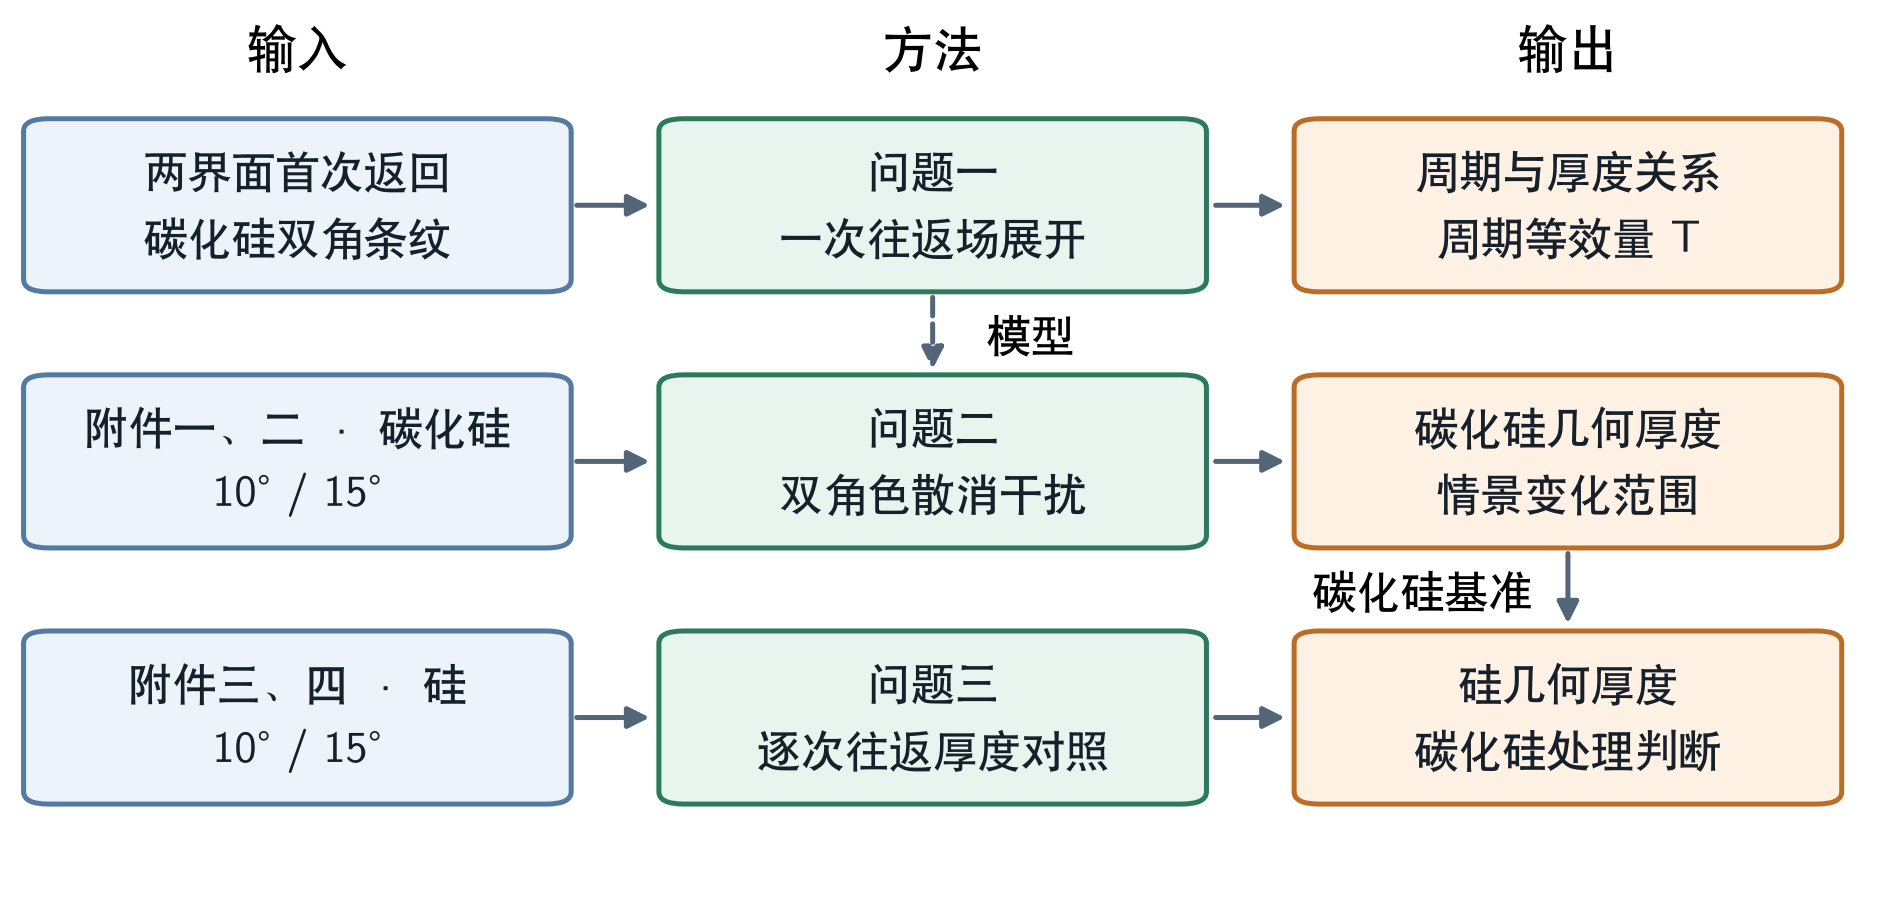
\includegraphics[width=0.8\textwidth,trim=0 38bp 0 0,clip]{../求解/公共/图片/全文思路图.png}
    \caption{四附件沿三问展开共同测厚路径}
    \label{fig:overall-route}
\end{figure}

总体组织吸收了高相关性的核对结果：两角原谱相关系数约为 $0.9987$，但来自同一块晶圆，并非独立厚度样本。原先以高相关性评价厚度可靠性的尝试，因而改为连续留段检验，即留出连续波段，用其观测检验双角预测。%
% src:交接/实验记录.json:50.现象;50.决定
% src:交接/数据档案.json:跨文件关系.两两全量核验.0.原始反射率皮尔逊相关系数

三问的结果按第\ref{sec:thickness-quantities}节的物理量定义区分；周期等效量为$19.54\ \mu\mathrm{m}$，表~\ref{tab:three-answers}将其与两种材料的测厚答案并列。%
% src:求解/问题1/结果/模型验证.json:真实附件诊断.表观光学厚度乘积_dq_微米

\begin{longtable}{>{\centering\arraybackslash}p{0.09\textwidth} >{\centering\arraybackslash}p{0.36\textwidth} >{\centering\arraybackslash}p{0.23\textwidth} >{\centering\arraybackslash}p{0.20\textwidth}}
\caption{三问回答的物理量与适用条件}\label{tab:three-answers}\\
\hline
问题 & 物理量 & 数值及单位 & 适用条件\\
\hline
\endfirsthead
\hline
问题 & 物理量 & 数值及单位 & 适用条件\\
\hline
\endhead
问题一 & 周期等效量 $T$ & $19.54\,\mu\mathrm{m}$ & 条纹周期折算\\
问题二 & 碳化硅几何厚度 & $10.80\,\mu\mathrm{m}$ & 非触边代表值\\
问题三 & 硅完整往返条件估计 & $2.17\,\mu\mathrm{m}$ & 给定经验色散\\
问题三 & 硅非概率条件包络 & $1.72$--$18.16\,\mu\mathrm{m}$ & 多情景联合范围\\
\hline
\end{longtable}
\nopagebreak[4]
\noindent{\small 注：硅点估计对应全量光谱；包络是多情景范围，不是置信区间。}
% src:求解/问题1/结果/模型验证.json:真实附件诊断.表观光学厚度乘积_dq_微米
% src:求解/问题2/结果/厚度结果.json:同片最佳厚度_微米;条件区间_微米
% src:求解/问题3/结果/回炉轮3候选/仲裁闭环/20260910_131501_81623_建模公式/厚度结果.json:核心指标.硅全量完整往返厚度_um;核心指标.碳化硅正式基准厚度_um
% src:求解/问题3/结果/回炉轮3候选/仲裁闭环/20260910_131501_81623_建模公式/厚度结果.json:核心指标.硅已计算条件包络下限_um;核心指标.硅已计算条件包络上限_um

碳化硅行采用透明两束与经验色散假设，代表值保留参数未碰到搜索边界的原估计。另有 $13.53\,\mu\mathrm{m}$ 的候选损失更低，但折射率已到搜索下界；分段重估、近优解及参数扰动构成的完整情景范围仍为 $0.64$--$18.11\,\mu\mathrm{m}$。
% src:求解/问题2/结果/厚度结果.json:同片最佳厚度_微米;同片最佳厚度的参考折射率;全量训练标准化损失;条件区间_微米;条件区间构造;条件区间组成
% src:求解/问题2/结果/验证.json:窗口与模型灵敏度.8.厚度_um;窗口与模型灵敏度.8.参考折射率;窗口与模型灵敏度.8.训练标准化损失
% src:求解/问题2/结果/搜索补查.json:代表点规则;补查最低损失候选.触边参数

周期等效量与几何厚度的换算条件统一见第\ref{sec:thickness-quantities}节。

入口、角度和结果对象被这样锁定后，后文即可先检查原始数据边界，再分别展开一次返回、双角估计与高阶往返的物理关系。
